% Phân công:
% - Nguyễn Xuân Cường (MSSV: 20237307) - trang 220-224
% - Nguyễn Minh Đức (MSSV: 20237313) - trang 225-229
% - Vũ Công Hiệp (MSSV: 20237328) - trang 230-234
% - Mục: 5.4 Confidence Regions and Simultaneous Comparisons of Component Means
% Vị trí viết nội dung: mỗi người thêm comment BEGIN/END phần của mình dưới dòng TODO.

\section{Confidence Regions and Simultaneous Comparisons of Component Means}

% TODO: Add content for Section 5.4.
% BEGIN Vũ Công Hiệp
 
\begin{figure}[htbp]
  \centering
  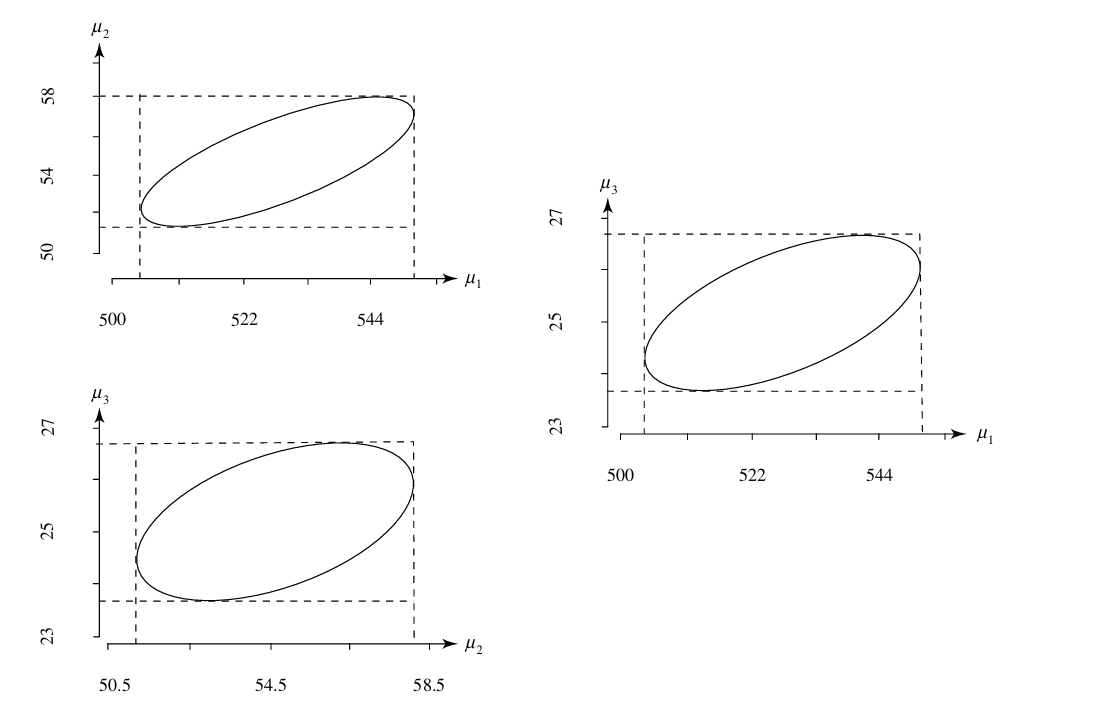
\includegraphics[width=0.7\textwidth]{figures/figure_5_3.png}
  \caption*{\textbf{Hình 5.3} Các elip tin cậy 95\% cho từng cặp trung bình và các khoảng $T^2$ đồng thời -- dữ liệu bài kiểm tra đại học.}
\end{figure}
 
Mặc dù trước khi lấy mẫu, khoảng tin cậy thứ $i$ có xác suất $1-\alpha$ bao phủ $\mu_i$, nhưng nói chung chúng ta không biết phải phát biểu như thế nào về xác suất để \emph{tất cả} các khoảng đều chứa các giá trị $\mu_i$ tương ứng. Như đã chỉ ra, xác suất này không phải là $1-\alpha$.
 
Để làm rõ hơn vấn đề này, hãy xét trường hợp đặc biệt trong đó các quan sát có phân phối chuẩn đồng thời và
 
\[
\boldsymbol{\Sigma}
=
\begin{bmatrix}
\sigma_{11} & 0 & \cdots & 0\\
0 & \sigma_{22} & \cdots & 0\\
\vdots & \vdots & \ddots & \vdots\\
0 & 0 & \cdots & \sigma_{pp}
\end{bmatrix}.
\]
 
Vì các quan sát trên biến thứ nhất độc lập với các quan sát trên biến thứ hai, và cứ như vậy, nên quy tắc nhân xác suất cho các biến cố độc lập có thể được áp dụng. Trước khi mẫu được chọn, ta có
 
\[
P[\text{tất cả các khoảng $t$ trong (5-27) đều chứa các } \mu_i]
=
(1-\alpha)(1-\alpha)\cdots(1-\alpha)
=
(1-\alpha)^p.
\]
 
Nếu $1-\alpha=0{,}95$ và $p=6$, xác suất này là
 
\[
(0{,}95)^6 \approx 0{,}74.
\]
 
% --- Tiếp nối: Confidence Regions and Simultaneous Comparisons of Component Means ---
 
Để đảm bảo xác suất $1-\alpha$ rằng tất cả các phát biểu về các trung bình thành phần đều đúng đồng thời, các khoảng cho từng thành phần phải rộng hơn các khoảng $t$ riêng lẻ. Mức độ rộng hơn bao nhiêu phụ thuộc vào cả $p$ và $n$, cũng như $1-\alpha$.
 
Với $1-\alpha=0{,}95$, $n=15$, $p=4$, các hệ số nhân của $\sqrt{s_{ii}/n}$ trong (5-24) và (5-27) lần lượt là
 
\[
\sqrt{\frac{p(n-1)}{n-p}F_{p,n-p}(0{,}05)}
=
\sqrt{\frac{4(14)}{11}(3{,}36)}
=
4{,}14
\]
 
và
 
\[
t_{n-1}(0{,}025)=2{,}145.
\]
 
Do đó, trong trường hợp này, các khoảng đồng thời rộng hơn $100(4{,}14-2{,}145)/2{,}145 \approx 93\%$ so với các khoảng suy ra từ phương pháp $t$ từng biến một (\emph{one-at-a-time}).
 
Bảng 5.3 đưa ra các hệ số nhân khoảng cách tới hạn cho các khoảng $t$ từng biến một được tính theo (5-21), cũng như các khoảng $T^2$ đồng thời tương ứng. Nói chung, độ rộng của các khoảng $T^2$ so với các khoảng $t$ tăng lên khi $p$ tăng (với $n$ cố định) và giảm đi khi $n$ tăng (với $p$ cố định).
 
\begin{table}[htbp]
    \centering
    \caption*{\textbf{Bảng 5.3} Hệ số nhân khoảng cách tới hạn cho các khoảng $t$ từng biến một và khoảng $T^2$ đồng thời với các giá trị $n$ và $p$ được chọn ($1-\alpha=0{,}95$).}
    \vspace{0.2cm}
 
    \begin{tabular}{c c c c}
        \toprule
        $n$
        & $t_{n-1}(0{,}025)$
        & \multicolumn{2}{c}{$
        \sqrt{\dfrac{(n-1)p}{n-p}F_{p,n-p}(0{,}05)}
        $} \\
        \cmidrule(lr){3-4}
        & & $p=4$ & $p=10$ \\
        \midrule
        15  & 2,145 & 4,14 & 11,52 \\
        25  & 2,064 & 3,60 & 6,39 \\
        50  & 2,010 & 3,31 & 5,05 \\
        100 & 1,970 & 3,19 & 4,61 \\
        $\infty$ & 1,960 & 3,08 & 4,28 \\
        \bottomrule
    \end{tabular}
\end{table}
 
Sự so sánh được ngụ ý trong Bảng 5.3 có phần không hoàn toàn công bằng, vì mức tin cậy gắn với bất kỳ tập hợp các khoảng $T^2$ nào, với $n$ và $p$ cố định, luôn là $0{,}95$; trong khi mức tin cậy tổng thể gắn với một tập hợp các khoảng $t$ riêng lẻ, cho cùng giá trị $n$, như chúng ta đã thấy, có thể nhỏ hơn $0{,}95$ rất nhiều.
 
Các khoảng $t$ từng biến một quá ngắn để duy trì mức tin cậy tổng thể cho các phát biểu riêng biệt về, chẳng hạn, tất cả $p$ trung bình. Tuy nhiên, đôi khi chúng ta vẫn xem chúng là thông tin tốt nhất có thể về một giá trị trung bình nếu đó là suy luận duy nhất cần thực hiện. Hơn nữa, nếu các khoảng $t$ từng biến một chỉ được tính toán khi kiểm định $T^2$ bác bỏ giả thuyết không, một số nhà nghiên cứu cho rằng chúng có thể phản ánh thông tin về các trung bình chính xác hơn so với các khoảng $T^2$.
 
Các khoảng $T^2$ quá rộng nếu chúng chỉ được áp dụng cho riêng $p$ trung bình thành phần. Để thấy rõ lý do, hãy xem xét elip tin cậy và các khoảng đồng thời được thể hiện trong Hình 5.2. Nếu $\mu_1$ nằm trong khoảng $T^2$ của nó và $\mu_2$ nằm trong khoảng $T^2$ của nó, thì $(\mu_1,\mu_2)$ nằm trong hình chữ nhật được tạo bởi hai khoảng này. Hình chữ nhật này chứa elip tin cậy và còn hơn thế nữa.
 
Elip tin cậy nhỏ hơn nhưng có xác suất $0{,}95$ bao phủ vectơ trung bình $\boldsymbol{\mu}$ với các trung bình thành phần $\mu_1$ và $\mu_2$. Do đó, xác suất bao phủ đồng thời hai trung bình riêng lẻ $\mu_1$ và $\mu_2$ của hình chữ nhật được tạo bởi các khoảng $T^2$ sẽ lớn hơn $0{,}95$.
 
Kết quả này dẫn chúng ta đến việc xem xét một cách tiếp cận thứ hai để thực hiện so sánh bội, được gọi là phương pháp Bonferroni.
 
\subsection*{Phương pháp so sánh bội Bonferroni}
 
Thông thường, sự chú ý chỉ giới hạn ở một số lượng nhỏ các phát biểu tin cậy riêng lẻ. Trong những tình huống này, ta có thể làm tốt hơn so với các khoảng đồng thời của Kết quả 5.3. Nếu số lượng $m$ các trung bình thành phần $\mu_i$ được chỉ định, hoặc các tổ hợp tuyến tính
\[
\mathbf{a}'\boldsymbol{\mu}
=
a_1\mu_1+a_2\mu_2+\cdots+a_p\mu_p,
\]
là nhỏ, ta có thể xây dựng các khoảng tin cậy đồng thời ngắn hơn (chính xác hơn) so với các khoảng $T^2$ đồng thời. Phương pháp thay thế này cho so sánh bội được gọi là \textit{phương pháp Bonferroni}, vì nó được phát triển từ một bất đẳng thức xác suất mang cùng tên.
 
Giả sử rằng, trước khi thu thập dữ liệu, ta cần thực hiện các phát biểu tin cậy về $m$ tổ hợp tuyến tính
\[
\mathbf{a}_1'\boldsymbol{\mu},
\mathbf{a}_2'\boldsymbol{\mu},
\ldots,
\mathbf{a}_m'\boldsymbol{\mu}.
\]
Gọi $C_i$ là một phát biểu tin cậy về giá trị của $\mathbf{a}_i'\boldsymbol{\mu}$ với
\[
P[C_i\text{ đúng}]=1-\alpha_i,
\qquad i=1,2,\ldots,m.
\]
Khi đó (xem Bài tập 5.6),
 
\begin{equation*}
\tag{5-28}
\begin{aligned}
P[\text{tất cả }C_i\text{ đều đúng}]
&=1-P[\text{ít nhất một }C_i\text{ sai}]\\
&\geq 1-\sum_{i=1}^{m}P(C_i\text{ sai})\\
&=1-\sum_{i=1}^{m}\bigl(1-P(C_i\text{ đúng})\bigr)\\
&=1-(\alpha_1+\alpha_2+\cdots+\alpha_m).
\end{aligned}
\end{equation*}
 
Bất đẳng thức (5-28), một trường hợp đặc biệt của bất đẳng thức Bonferroni, cho phép nhà nghiên cứu kiểm soát tỷ lệ sai số tổng thể $\alpha_1+\alpha_2+\cdots+\alpha_m$, bất kể cấu trúc tương quan đằng sau các phát biểu tin cậy. Ngoài ra còn có sự linh hoạt trong việc kiểm soát tỷ lệ sai số cho một nhóm các phát biểu quan trọng, và cân bằng bằng một lựa chọn khác cho các phát biểu ít quan trọng hơn.
 
Ta phát triển các ước lượng khoảng đồng thời cho tập hạn chế gồm các thành phần $\mu_i$ của $\boldsymbol{\mu}$. Do không có thông tin về tầm quan trọng tương đối của các thành phần này, ta xét các khoảng $t$ riêng lẻ
\[
\bar{x}_i
\pm
t_{n-1}\left(\frac{\alpha_i}{2}\right)
\sqrt{\frac{s_{ii}}{n}},
\qquad i=1,2,\ldots,m,
\]
với $\alpha_i=\alpha/m$. Vì
\[
P\left[
\bar{X}_i
\pm
t_{n-1}\left(\frac{\alpha}{2m}\right)
\sqrt{\frac{S_{ii}}{n}}
\text{ chứa }\mu_i
\right]
=
1-\frac{\alpha}{m},
\qquad i=1,2,\ldots,m,
\]
nên từ (5-28) ta có
 
\[
P\left[
\bar{X}_i
\pm
t_{n-1}\left(\frac{\alpha}{2m}\right)
\sqrt{\frac{S_{ii}}{n}}
\text{ chứa }\mu_i,\ \forall i
\right]
\geq
1-
\underbrace{\left(
\frac{\alpha}{m}
+\frac{\alpha}{m}
+\cdots+
\frac{\alpha}{m}
\right)}_{m\text{ số hạng}}
=
1-\alpha.
\]
 
Do đó, với mức tin cậy tổng thể lớn hơn hoặc bằng $1-\alpha$, ta có thể đưa ra $m=p$ phát biểu sau:
 
\begin{equation*}
\tag{5-29}
\begin{aligned}
\bar{x}_1
-
t_{n-1}\left(\frac{\alpha}{2p}\right)
\sqrt{\frac{s_{11}}{n}}
&\leq
\mu_1
\leq
\bar{x}_1
+
t_{n-1}\left(\frac{\alpha}{2p}\right)
\sqrt{\frac{s_{11}}{n}}
\\[4pt]
\bar{x}_2
-
t_{n-1}\left(\frac{\alpha}{2p}\right)
\sqrt{\frac{s_{22}}{n}}
&\leq
\mu_2
\leq
\bar{x}_2
+
t_{n-1}\left(\frac{\alpha}{2p}\right)
\sqrt{\frac{s_{22}}{n}}
\\[-1pt]
&\vdots
\\[-1pt]
\bar{x}_p
-
t_{n-1}\left(\frac{\alpha}{2p}\right)
\sqrt{\frac{s_{pp}}{n}}
&\leq
\mu_p
\leq
\bar{x}_p
+
t_{n-1}\left(\frac{\alpha}{2p}\right)
\sqrt{\frac{s_{pp}}{n}}
\end{aligned}
\end{equation*}
 
Các phát biểu trong (5-29) có thể được so sánh với các phát biểu trong (5-24).
Giá trị tới hạn $t_{n-1}(\alpha/2p)$ thay thế cho
$\sqrt{(n-1)\,p\,F_{p,n-p}(\alpha)/(n-p)}$, nhưng ngoài điểm thay thế này ra,
các khoảng có cùng cấu trúc.
 
\textbf{Ví dụ 5.6 (Xây dựng các khoảng tin cậy đồng thời Bonferroni và so sánh
chúng với các khoảng $T^2$)}
Hãy quay lại với dữ liệu bức xạ lò vi sóng trong Ví dụ 5.3 và 5.4. Chúng ta sẽ
tìm các khoảng tin cậy đồng thời Bonferroni 95\% cho các giá trị trung bình
$\mu_1$ và $\mu_2$ của căn bậc bốn các phép đo khi đóng cửa và khi mở cửa, với
$\alpha_i = 0{,}05/2$, $i = 1, 2$. Chúng ta sử dụng các kết quả trong Ví dụ 5.3,
lưu ý rằng $n = 42$ và $t_{41}(0{,}05/2(2)) = t_{41}(0{,}0125) = 2{,}327$, để thu
được:
 
\begin{gather*}
  \bar{x}_1 \pm t_{41}(0{,}0125)\sqrt{\frac{s_{11}}{n}}
  = 0{,}564 \pm 2{,}327\sqrt{\frac{0{,}0144}{42}}
  \quad \text{hay} \quad 0{,}521 \le \mu_1 \le 0{,}607 \\[1ex]
  \bar{x}_2 \pm t_{41}(0{,}0125)\sqrt{\frac{s_{22}}{n}}
  = 0{,}603 \pm 2{,}327\sqrt{\frac{0{,}0146}{42}}
  \quad \text{hay} \quad 0{,}560 \le \mu_2 \le 0{,}646
\end{gather*}
 
Hình 5.4 cho thấy các khoảng tin cậy đồng thời $T^2$ 95\% cho $\mu_1, \mu_2$ từ
Hình 5.2, cùng với các khoảng Bonferroni 95\% tương ứng. Đối với mỗi trung bình
thành phần, khoảng Bonferroni nằm trong khoảng $T^2$. Do đó, vùng hình chữ nhật
(chung) được tạo bởi hai khoảng Bonferroni được chứa trong vùng hình chữ nhật
được tạo bởi hai khoảng $T^2$. Nếu chúng ta chỉ quan tâm đến các trung bình
thành phần, các khoảng Bonferroni cung cấp các ước lượng chính xác hơn (khoảng
hẹp hơn) so với khoảng $T^2$. Mặt khác, miền tin cậy 95\% đối với
$\boldsymbol{\mu}$ cung cấp các giá trị hợp lý cho các cặp $(\mu_1, \mu_2)$ khi
tính đến tương quan giữa các biến được đo. \hfill $\blacksquare$
 
\begin{figure}[htbp]
  \centering
  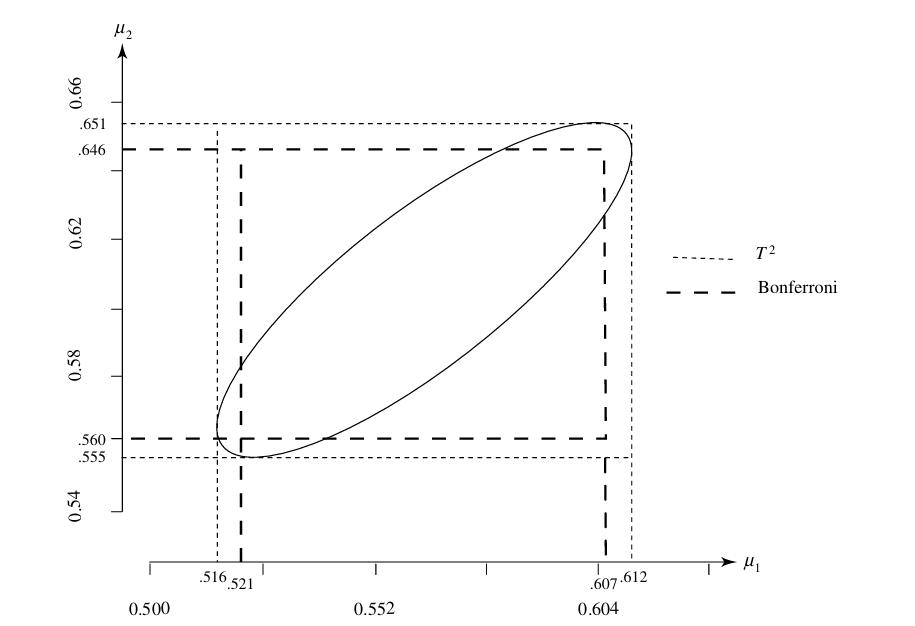
\includegraphics[width=0.7\textwidth]{figures/figure_5_4.png}
  \caption*{\textbf{Hình 5.4} Các khoảng tin cậy đồng thời $T^2$ 95\% và Bonferroni 95\% cho các trung bình thành phần -- dữ liệu bức xạ lò vi sóng.}
\end{figure}
 
%----------------------------------------------------------------------
% So sánh độ dài Bonferroni và T^2
%----------------------------------------------------------------------
Các khoảng Bonferroni đối với các tổ hợp tuyến tính $\mathbf{a}'\boldsymbol{\mu}$
và các khoảng $T^2$ tương tự (nhắc lại Kết quả 5.3) có cùng dạng tổng quát:
\[
  \mathbf{a}'\bar{\mathbf{X}} \pm (\text{giá trị tới hạn})
  \sqrt{\frac{\mathbf{a}'\mathbf{S}\mathbf{a}}{n}}
\]
 
Do đó, trong mọi trường hợp mà $\alpha_i = \alpha/m$,
\begin{equation*}
  \tag{5-30}
  \frac{\text{Độ dài khoảng Bonferroni}}{\text{Độ dài khoảng } T^2}
  = \frac{t_{n-1}(\alpha/2m)}
         {\sqrt{\dfrac{p(n-1)}{n-p}\,F_{p,n-p}(\alpha)}}
\end{equation*}
và tỷ số này không phụ thuộc vào các đại lượng ngẫu nhiên $\bar{\mathbf{X}}$
và $\mathbf{S}$. Như chúng ta đã chỉ ra, đối với một số lượng nhỏ $m$ các hàm
tham số được chỉ định trước $\mathbf{a}'\boldsymbol{\mu}$, các khoảng Bonferroni
sẽ luôn ngắn hơn. Bảng 5.4 cho thấy mức độ ngắn hơn đối với các giá trị $n$ và
$p$ được chọn.
 
\begin{table}[htbp]
\centering
\caption*{\textbf{Bảng 5.4} (Độ dài khoảng Bonferroni)/(Độ dài khoảng $T^2$) với $1-\alpha = 0{,}95$ và $\alpha_i = 0{,}05/m$}
\vspace{0.3em}
\begin{tabular}{c|ccc}
\hline
 & \multicolumn{3}{c}{$m = p$} \\ \cline{2-4}
$n$ & 2 & 4 & 10 \\ \hline
15 & 0,88 & 0,69 & 0,29 \\
25 & 0,90 & 0,75 & 0,48 \\
50 & 0,91 & 0,78 & 0,58 \\
100 & 0,91 & 0,80 & 0,62 \\
$\infty$ & 0,91 & 0,81 & 0,66 \\
\hline
\end{tabular}
\end{table}
 
Từ Bảng 5.4, chúng ta thấy rằng phương pháp Bonferroni cho các khoảng ngắn hơn
khi $m = p$. Vì chúng dễ áp dụng và cho các khoảng tin cậy tương đối ngắn cần
thiết cho suy diễn thống kê, chúng ta thường sẽ áp dụng các khoảng $t$ đồng thời
dựa trên phương pháp Bonferroni.
% END Vũ Công Hiệp